\documentclass[12pt,spanish]{article}
\usepackage[spanish]{babel}
\selectlanguage{spanish}
\usepackage[utf8x]{inputenc}
\usepackage{graphicx}
\graphicspath{{images/}}
\usepackage{amsfonts}
\usepackage{float}
\usepackage{url}
\usepackage{fancyhdr}
\usepackage{vmargin}
\usepackage{multirow}
\usepackage{chngpage}
\usepackage{hyperref}
\usepackage{listing}
\usepackage{subcaption}
\usepackage{amsmath}

\usepackage[
    type={CC},
    modifier={by-nc-sa},
    version={4.0},
]{doclicense}

\hypersetup{
    colorlinks=true,
    linkcolor=blue,
    filecolor=magenta,
    urlcolor=cyan,
}

% para codigo
\usepackage{listings}
\usepackage{xcolor}



%% configuración de listings

\definecolor{listing-background}{HTML}{F7F7F7}
\definecolor{listing-rule}{HTML}{B3B2B3}
\definecolor{listing-numbers}{HTML}{B3B2B3}
\definecolor{listing-text-color}{HTML}{000000}
\definecolor{listing-keyword}{HTML}{435489}
\definecolor{listing-identifier}{HTML}{435489}
\definecolor{listing-string}{HTML}{00999A}
\definecolor{listing-comment}{HTML}{8E8E8E}
\definecolor{listing-javadoc-comment}{HTML}{006CA9}

\lstdefinestyle{eisvogel_listing_style}{
  language         = python,
%$if(listings-disable-line-numbers)$
%  xleftmargin      = 0.6em,
%  framexleftmargin = 0.4em,
%$else$
  numbers          = left,
  xleftmargin      = 0em,
 framexleftmargin = 0em,
%$endif$
  backgroundcolor  = \color{listing-background},
  basicstyle       = \color{listing-text-color}\small\ttfamily{}\linespread{1.15}, % print whole listing small
  breaklines       = true,
  frame            = single,
  framesep         = 0.19em,
  rulecolor        = \color{listing-rule},
  frameround       = ffff,
  tabsize          = 4,
  numberstyle      = \color{listing-numbers},
  aboveskip        = 1.0em,
  belowskip        = 0.1em,
  abovecaptionskip = 0em,
  belowcaptionskip = 1.0em,
  keywordstyle     = \color{listing-keyword}\bfseries,
  classoffset      = 0,
  sensitive        = true,
  identifierstyle  = \color{listing-identifier},
  commentstyle     = \color{listing-comment},
  morecomment      = [s][\color{listing-javadoc-comment}]{/**}{*/},
  stringstyle      = \color{listing-string},
  showstringspaces = false,
  escapeinside     = {/*@}{@*/}, % Allow LaTeX inside these special comments
  literate         =
  {á}{{\'a}}1 {é}{{\'e}}1 {í}{{\'i}}1 {ó}{{\'o}}1 {ú}{{\'u}}1
  {Á}{{\'A}}1 {É}{{\'E}}1 {Í}{{\'I}}1 {Ó}{{\'O}}1 {Ú}{{\'U}}1
  {à}{{\`a}}1 {è}{{\'e}}1 {ì}{{\`i}}1 {ò}{{\`o}}1 {ù}{{\`u}}1
  {À}{{\`A}}1 {È}{{\'E}}1 {Ì}{{\`I}}1 {Ò}{{\`O}}1 {Ù}{{\`U}}1
  {ä}{{\"a}}1 {ë}{{\"e}}1 {ï}{{\"i}}1 {ö}{{\"o}}1 {ü}{{\"u}}1
  {Ä}{{\"A}}1 {Ë}{{\"E}}1 {Ï}{{\"I}}1 {Ö}{{\"O}}1 {Ü}{{\"U}}1
  {â}{{\^a}}1 {ê}{{\^e}}1 {î}{{\^i}}1 {ô}{{\^o}}1 {û}{{\^u}}1
  {Â}{{\^A}}1 {Ê}{{\^E}}1 {Î}{{\^I}}1 {Ô}{{\^O}}1 {Û}{{\^U}}1
  {œ}{{\oe}}1 {Œ}{{\OE}}1 {æ}{{\ae}}1 {Æ}{{\AE}}1 {ß}{{\ss}}1
  {ç}{{\c c}}1 {Ç}{{\c C}}1 {ø}{{\o}}1 {å}{{\r a}}1 {Å}{{\r A}}1
  {€}{{\EUR}}1 {£}{{\pounds}}1 {«}{{\guillemotleft}}1
  {»}{{\guillemotright}}1 {ñ}{{\~n}}1 {Ñ}{{\~N}}1 {¿}{{?`}}1
  {…}{{\ldots}}1 {≥}{{>=}}1 {≤}{{<=}}1 {„}{{\glqq}}1 {“}{{\grqq}}1
  {”}{{''}}1
}
\lstset{style=eisvogel_listing_style}


\usepackage[default]{source sans pro}

\setmarginsrb{2 cm}{1 cm}{2 cm}{2 cm}{1 cm}{1.5 cm}{1 cm}{1.5 cm}
\title{Práctica 1:\\
Máscaras y derivadas  \hspace{0.05cm} }
\author{Ángel Cabeza Martín}
\date{\today}

\renewcommand*\contentsname{hola}

\makeatletter
\let\thetitle\@title
\let\theauthor\@author
\let\thedate\@date
\makeatother

\pagestyle{fancy}
\fancyhf{}
\rhead{\theauthor}
\lhead{\thetitle}
\cfoot{\thepage}

\begin{document}

%%%%%%%%%%%%%%%%%%%%%%%%%%%%%%%%%%%%%%%%%%%%%%%%%%%%%
\begin{titlepage}
 
 
\newlength{\centeroffset}
\setlength{\centeroffset}{-0.5\oddsidemargin}
\addtolength{\centeroffset}{0.5\evensidemargin}
\thispagestyle{empty}

\noindent\hspace*{\centeroffset}

\centering
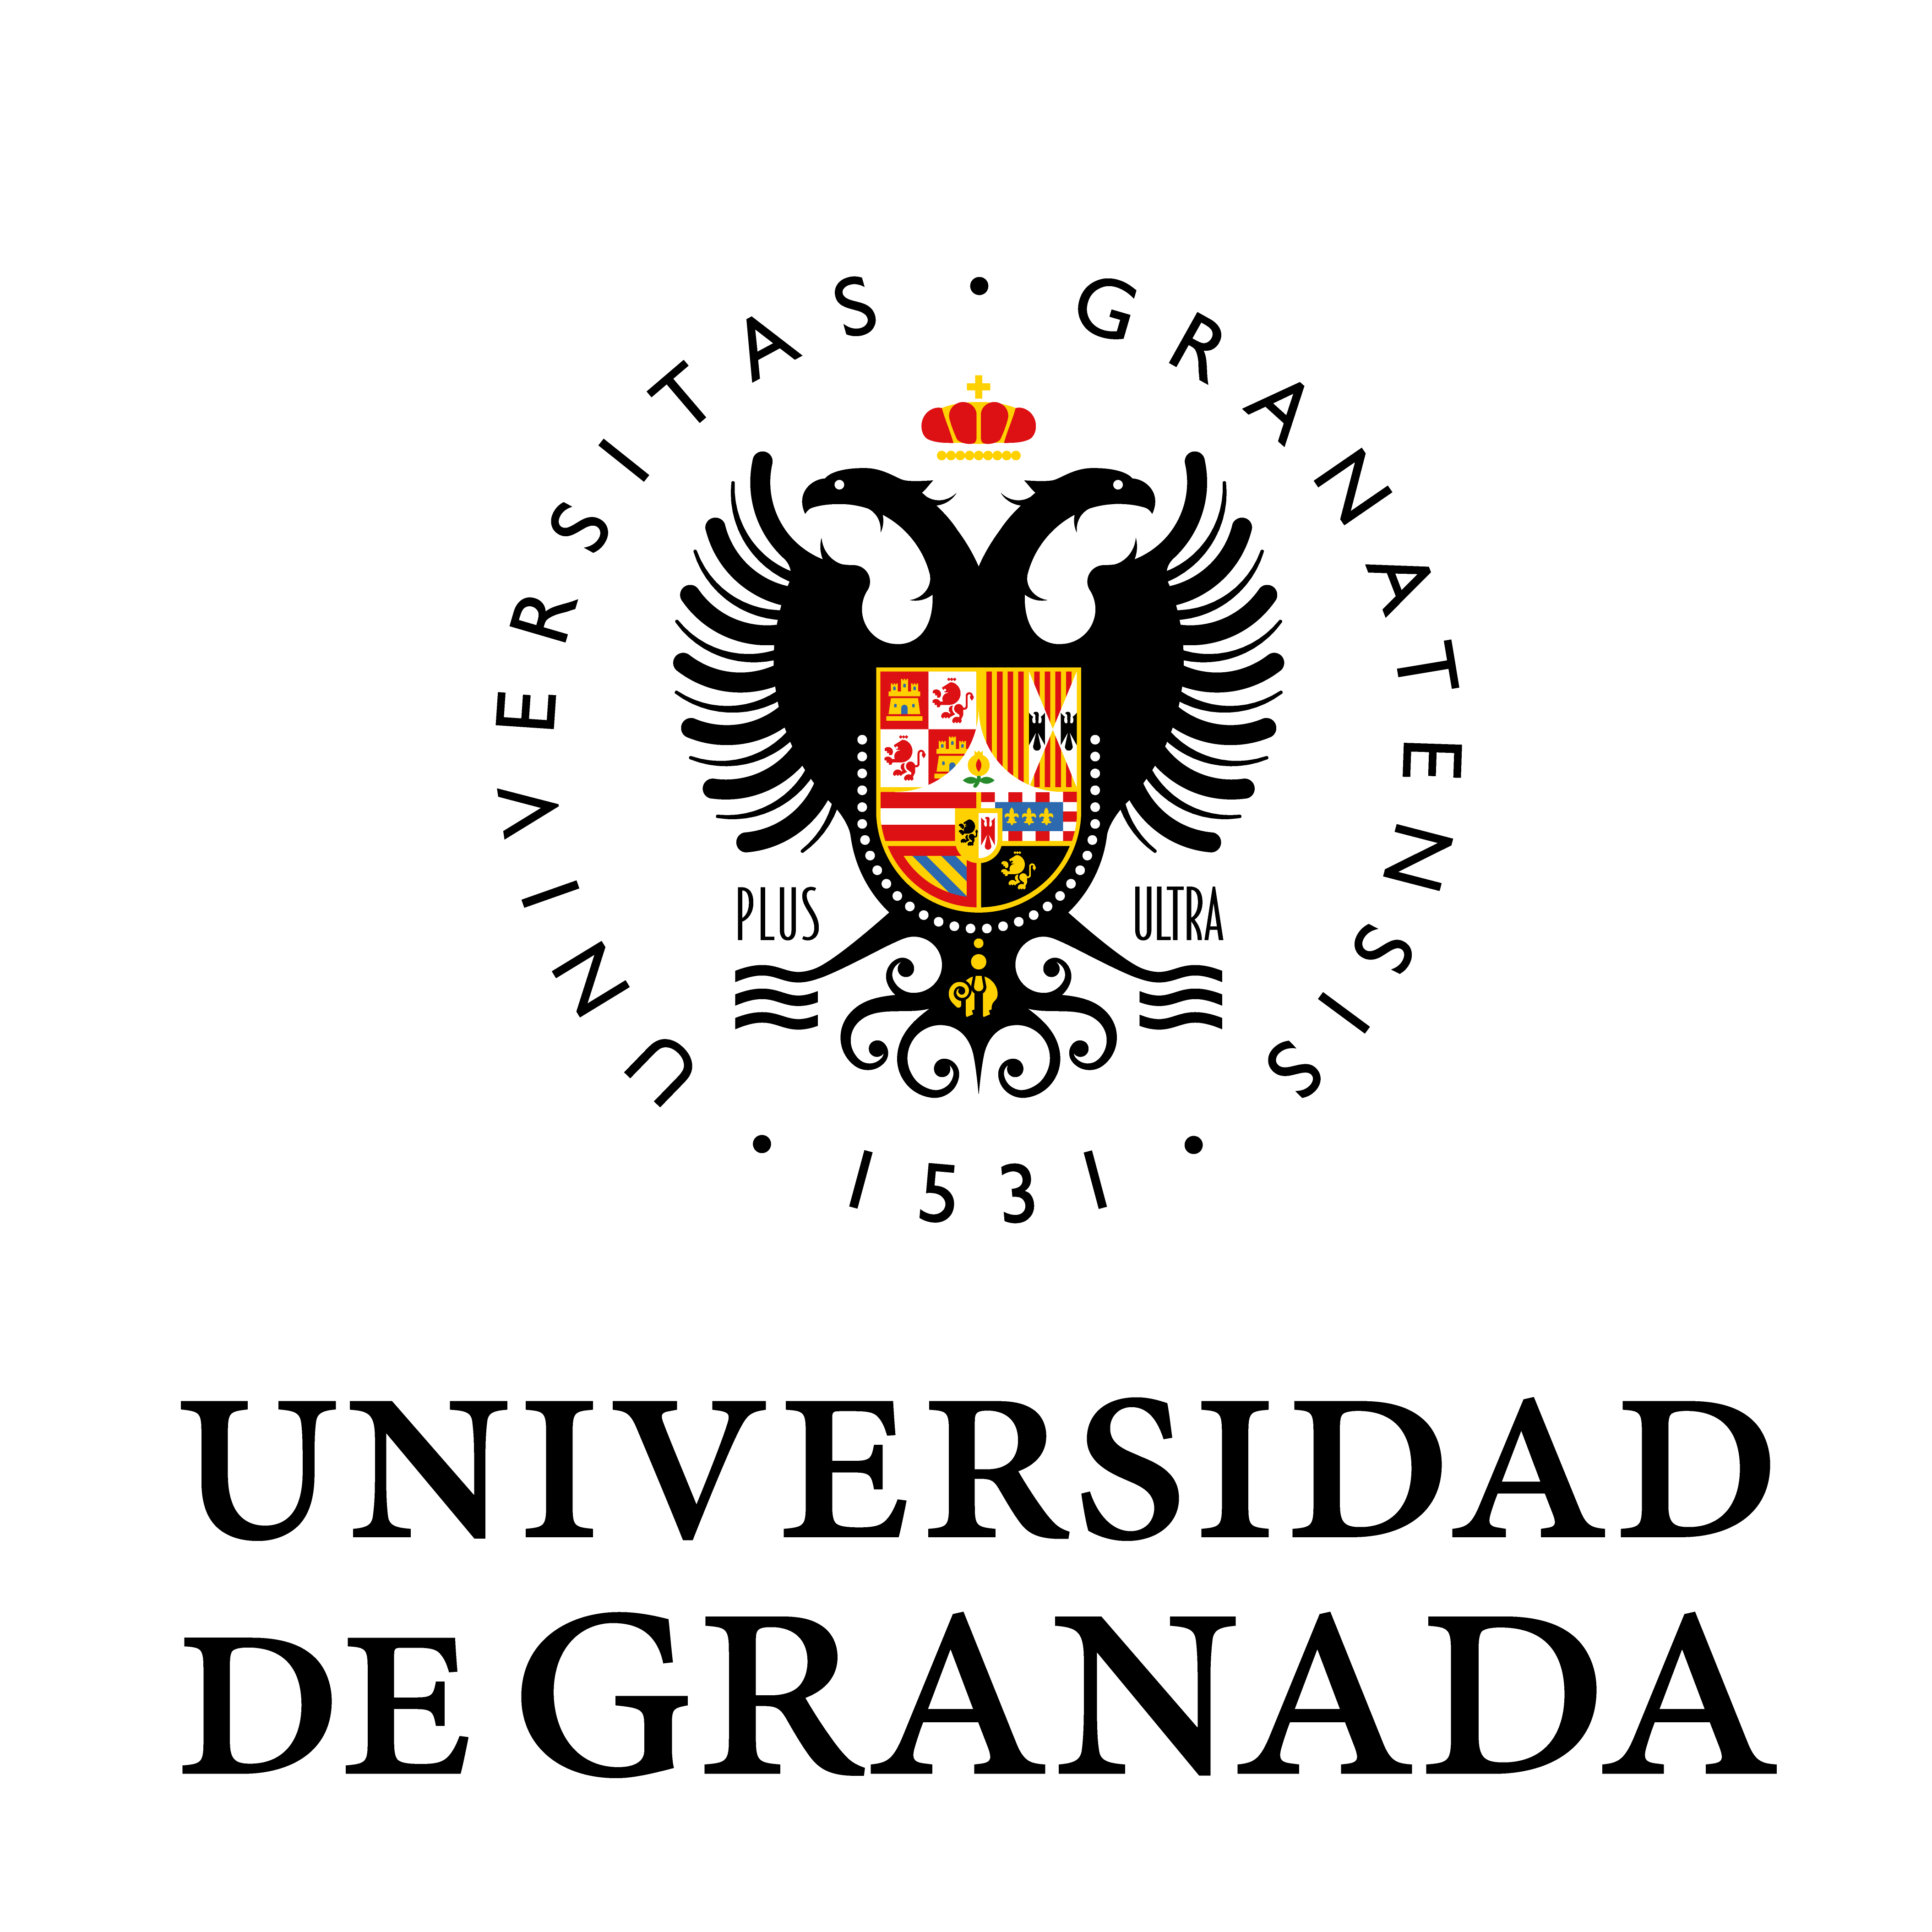
\includegraphics[width=0.9\textwidth]{./imagenes_memoria/ugr.png}\\[0.5cm]

\textsc{ \Large Práctica 1\\[0.2cm]}
\textsc{ \Large Ángel Cabeza Martín}\\
\textsc{ \Large 75571222F}\\
\textsl{ angelcabeza@correo.ugr.es}\\[0.5cm]
% Upper part of the page
% 
% Title
{\Huge\bfseries Máscaras y Derivadas\\
}
\noindent\rule[-1ex]{\textwidth}{2pt}\\[3.5ex]
{\large\bfseries Visión por Computador}
\end{titlepage}

%%%%%%%%%%%%%%%%%%%%%%%%%%%%%%%%%%%%%%%%%%%%%%%%%%%%%

\tableofcontents
\pagebreak
%%%%%%%%%%%%%%%%%%%%%%%%%%%%%%%%%%%%%%%%%%%%%%%%%%%%%

\section*{Introducción}
En esta práctica trabajaremos los filtros de máscaras, con el objetivo de extraer información significativa de imágenes y aprender el uso de las distintas propiedades de la función Gaussiana.\newline 

Esta práctica se centra en comparar nuestra implementación, hecha siguiendo la teoría, con la de OpenCV que se centra en buscar el máximo rendimiento obteniendo a su vez resultados aceptables, por ello todos los ejercicios estarán implementados sin usar ninguna función de OpenCV y solo usaremos estas por motivos comparativos.\\


Por último, quiero aclarar que en esta memoria no me voy a centrar en explicar cómo he desarrollado mi código, si no en las decisiones que he tomado para desarrollar la práctica y los conceptos teóricos que me han guiado para tomar esas decisiones.


\section{Ejercicio 1: Máscaras}
Este ejercicio trata sobre el cálculo de las máscaras Gaussianas que usaremos durante toda la práctica, la aplicación de estas para realizar una convolución y  para calcular un filtro Laplaciano y también aprenderemos cómo calcular máscaras a partir del kernel binomial. Además durante todos los apartados haremos una comparación entre nuestra implementación y la de OpenCV.

\subsection{Máscaras Discretas 1D}
Para calcular las distintas máscaras he implementado tres funciones:
\begin{enumerate}
	\item Función Gaussiana: Devuelve el valor de la función Gaussiana en un punto concreto para un sigma dado.
	\item Primera derivada de la función Gaussiana: devuelve el valor de la primera derivada de la Gaussiana para un punto concreto y un sigma dado
	\item Segunda derivada de la función Gaussiana: devuelve el valor de la segunda derivada de la Gaussiana para un punto concreto y un sigma dado
\end{enumerate}

Para la implementación de estas funciones, cogemos la expresión de la Gausiana y evaluamos el punto dado (he obviado la constante $c$ porque no influye en el cálculo):

\pagebreak

\begin{figure}
	\centering
	\[f(x) = c \cdot e^{-\frac{x²}{2\sigma²}} \]
	\caption{Función Gaussiana.}
	\label{f_gaussiana}
\end{figure}


Y para las derivadas simplemente hay que calcular las distintas derivadas de esta función respecto de $x$: 

\begin{figure}[H]
	\centering
	\[f'(x) = -\frac{x e^{-\frac{x²}{2 \cdot \sigma²}}}{\sigma²} \]
	\caption{Primera derivada de la Gaussiana.}
	\label{1d_gaussiana}
\end{figure}

\begin{figure}[H]
	\centering
	\[f''(x) = \frac{(x² - \sigma²) \cdot e^{-\frac{x²}{2*\sigma²}}}{\sigma⁴} \]
	\caption{Segunda derivada de la Gaussiana.}
	\label{2d_gaussiana}
\end{figure}

Una vez implementadas estas funciones, he creado la función \texttt{kernelGaussiano1D} que recibe como argumentos la función gaussiana a evaluar (por defecto sin derivada),un sigma y un tamaño de máscara. Estos dos últimos parámetros son opcionales pero siempre se tiene que dar por lo menos uno de ellos, si no el programa te advertirá del error y parará. Si se proporciona únicamente uno de ellos, el otro se calcula con la fórmula de \ref{f_sigma_tam}. \\

Una vez calculado el sigma o el tamaño de la máscara, evaluaremos la función pasada como argumento (la Gaussiana, la 1º derivada de la Gaussiana o la 2º derivada de la Gaussiana) en el intervalo [-T//2,T//2]. Si la función usada es la Gaussiana, normalizaremos la máscara diviendo cada valor de la máscara entre la suma de todos los valores de la máscara, si la función usada es la primera derivada de la Gaussiana multiplicaremos la máscara por $\sigma$ y si es la segunda derivada de la Gaussiana multiplicaremos la máscara por $\sigma²$. Las dervidas se multiplican por $\sigma$ para acentuar los cambios de intensidad de la señal y que estos no se pierdan al derivar. 

\begin{figure}[H]
	\centering
	\[ 2 \cdot [3 \cdot \sigma] + 1 = T \]
	\caption{Fórmula para calcular sigma y T}
	\label{f_sigma_tam}
\end{figure}

\pagebreak

Utilizamos esta fórmula ya que nos asegura que el tamaño de la máscara es al menos $3 \cdot \sigma$ y que dado un sigma este tamaño es impar. Ambas situaciones vimos en teoría que eran convenientes. \\

Tras calcular las máscaras de tamaño 5,7 y 9 y comparar los resultados con las máscaras calculadas por la función \texttt{getDerivKernel} de OpenCV hemos obtenido los resultados de las figuras \ref{mask_t5} \ref{mask_1d_t5} \ref{mask_2d_t5} \ref{mask_t7} \ref{mask_1d_t7} \ref{mask_2d_t7} \ref{mask_t9} \ref{mask_1d_t9} \ref{mask_2d_t9}. Como vemos las máscaras no son iguales, observamos dos grandes diferencias:

\begin{enumerate}
	\item Las máscaras de la primera derivada están invertidas.
	\item Cuanto mayor es el tamaño de la máscara, menor es el rango de valores en nuestras máscaras y mayor en las máscaras de getDerivKernels (este suceso está atenuado ya que las máscaras de getDerivKernels se encuentran normalizadas para favorecer la visualización).
\end{enumerate}

La primera diferencia no es importante porque las máscaras son simétricas por lo que ambas máscaras suman 0. La segunda derivada se debe a que OpenCV no efectúa un kernel Gaussiano como tal, hace una aproximación usando los operadores Sobel o Scharr, pero la forma es la misma ya que los 3 filtros realizan la misma función. Por lo tanto, nuestras máscaras son más exactas pero las de OpenCV son computacionalmente más rápidas.

\begin{figure}[H]
	\centering
	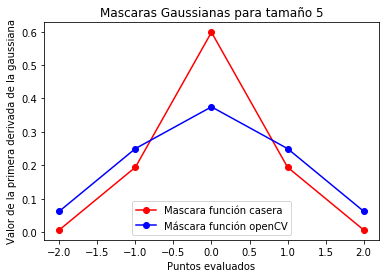
\includegraphics[width=12cm, scale=1]{./imagenes_memoria/1_t5.png}
	\caption{Comparativa de las máscaras Gaussianas de tamaño 5 de getDerivKernels y nuestra función}
	\label{mask_t5}
\end{figure}

\begin{figure}[H]
	\centering
	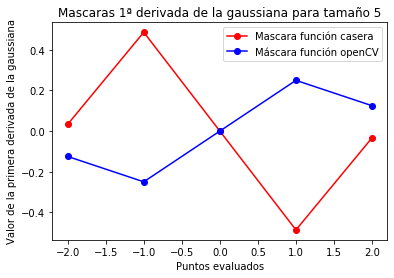
\includegraphics[width=12cm, scale=1]{./imagenes_memoria/1d_t5.png}
	\caption{Comparativa de las máscaras de 1ª derivada de tamaño 5 de getDerivKernels y nuestra función}
	\label{mask_1d_t5}
\end{figure}

\begin{figure}[H]
	\centering
	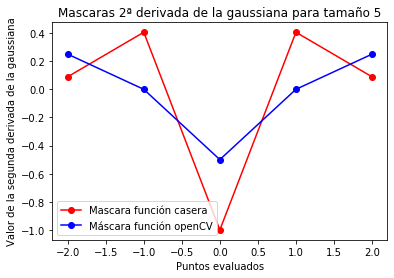
\includegraphics[width=12cm]{./imagenes_memoria/2d_t5.png}
	\caption{Comparativa de las máscaras de 2ª derivada de tamaño 5 de getDerivKernels y nuestra función}
	\label{mask_2d_t5}
\end{figure}

\begin{figure}[H]
	\centering
	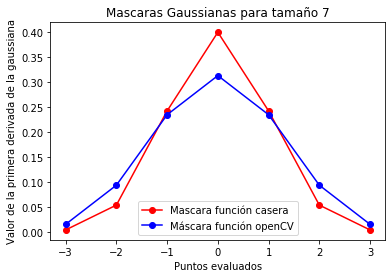
\includegraphics[width=12cm, scale=1]{./imagenes_memoria/1_t7.png}
	\caption{Comparativa de las máscaras Gaussianas de tamaño 7 de getDerivKernels y nuestra función}
	\label{mask_t7}
\end{figure}

\begin{figure}[H]
	\centering
	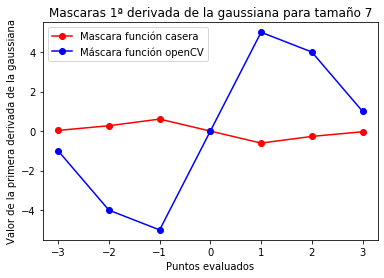
\includegraphics[width=12cm]{./imagenes_memoria/1d_t7.png}
	\caption{Comparativa de las máscaras de 1ª derivada de tamaño 7 de getDerivKernels y nuestra función}
	\label{mask_1d_t7}
\end{figure}

\begin{figure}[H]
	\centering
	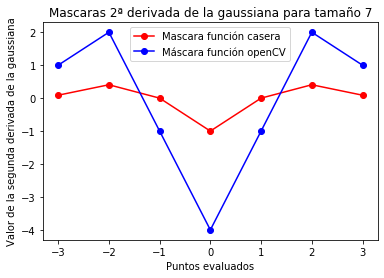
\includegraphics[width=12cm]{./imagenes_memoria/2d_t7.png}
	\caption{Comparativa de las máscaras de 2ª derivada de tamaño 7 de getDerivKernels y nuestra función}
	\label{mask_2d_t7}
\end{figure}

\begin{figure}[H]
	\centering
	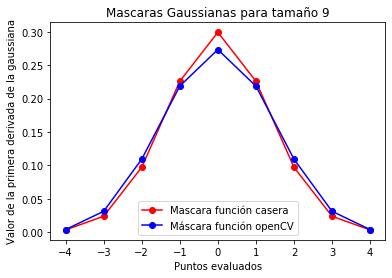
\includegraphics[width=12cm, scale=1]{./imagenes_memoria/1_t9.png}
	\caption{Comparativa de las máscaras Gaussianas de tamaño 9 de getDerivKernels y nuestra función}
	\label{mask_t9}
\end{figure}

\begin{figure}[H]
	\centering
	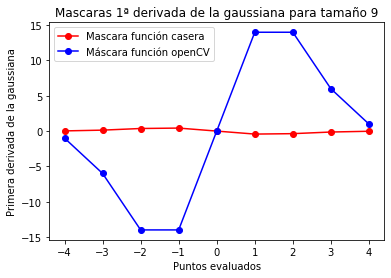
\includegraphics[width=12cm]{./imagenes_memoria/1d_t9.png}
	\caption{Comparativa de las máscaras de 1ª derivada de tamaño 9 de getDerivKernels y nuestra función}
	\label{mask_1d_t9}
\end{figure}

\begin{figure}[H]
	\centering
	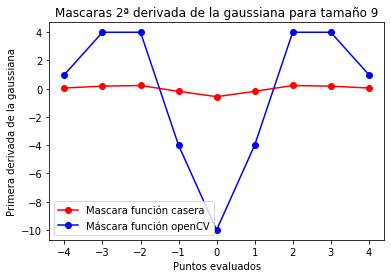
\includegraphics[width=12cm]{./imagenes_memoria/2d_t9.png}
	\caption{Comparativa de las máscaras de 2ª derivada de tamaño 9 de getDerivKernels y nuestra función}
	\label{mask_2d_t9}
\end{figure}

\subsection{Kernel binomial}
En este ejercicio se nos pide calcular las máscaras de tamaño 5 y 7, tanto de alisamiento como de derivada, a partir de la aproximación binomial de la Gaussiana ([1,2,1]) y la máscara de derivada de orden 3 ([-1,0,1]. \\

Para general la aproximación binomial hay que convolucionar la máscara del primer nivel de la aproximación ([1,2,1] para el caso de filtro Gaussiano) con la máscara de longitud que se desee (N) y el resultado de la convolución dará lugar a la máscara del nivel N+2 (veasé figura \ref{aproximacion_binomial}). De esta forma para calcular las mascaras de alisamiento de longitud 5 nos bastará realizar una convolución entre la máscara de tamaño 3 ([1,2,1]y ella misma y para obtener la máscara de longitud 7 tendremos que hacer una convolución entre la máscara de longitud 5 (que acabamos de calcular) y la de longitud 3. Para las derivadas hay que seguir el mismo proceso pero la máscara de longitud 3 es [-1,0,1].

\begin{figure}[H]
	\centering
	\begin{tabular}{|c | c | c |}
		\hline
		Longitud & Máscara & Área \\ \hline
		3 & [1,2,1] & 96.6 $\%$ \\ \hline
		5 & [1,4,6,4,1] & 98.76$\%$ \\ \hline
		7 & [1,6,15,20,15,6,1] & 98.58$\%$ \\ \hline
		9 & [1,8,28,56,70,56,28,8,1] & 99.85$\%$\\ \hline
	\end{tabular}
	\caption{Aproximación binomial}
	\label{aproximacion_binomial}
\end{figure}

Una vez entendido esto para aplicar la convolución he utilizado la funcion de numpy \texttt{convolve} ya que en este apartado aún no he programado mi propia función de convolución y he obtenido los siguientes resultados:

\begin{lstlisting}[frame=single]
Kernel alisamiento lon 5:  [1 4 6 4 1]
Kernel alisamiento lon 7:  [ 1  6 15 20 15  6  1]
Kernel derivada lon 5:  [-1 -2  0  2  1]
Kernel derivada lon 7:  [-1 -4 -5  0  5  4  1]
Kernel tam 9 alisamiento por OpenCV:  [[ 1.  8. 28. 56. 70. 56. 28.  8.  1.]]
Kernel tam 9 derivada por OpenCV:  [[ -1.  -6. -14. -14.   0.  14.  14.   6.   1.]]
Kernel tam 9 alisamiento calculado por mi :  [ 1  8 28 56 70 56 28  8  1]
Kernel tam 9 derivada calculado por mi :  [ -1  -6 -14 -14   0  14  14   6   1]
\end{lstlisting}

Como vemos getDerivKernels utiliza la aproximación binomial para calcular las máscaras. Esto lo hace para ahorrarse tiempo de cómputo a coste de perder cierta precisión.

\subsection{Convolución}
En este ejercicio se nos pide realizar una convolución en 2D, a partir de dos máscaras 1D. Para ello he implementado las siguientes funciones:

\begin{itemize}
	\item aniadeborde: Recibe como argumentos una imagen y la máscara con la que se va a convolucionar. Esta función hace uso del método CopyMakeBorder de OpenCV para añadir un borde con un tamaño igual a la mitad de la longitud de la máscara.
	\item convolucionar: esta función recibe una imagen (con el borde ya añadido) y dos máscaras, una con la convolucionar por filas y otra por columnas (lo he hecho así porque me facilitaba el siguiente ejercicio pero realmente se podría hacer con una sola) y devuelve la imagen convolucionada.
	\item Además me he servido de las funciones creadas en la práctica 0 para leer imágenes, dibujarlas etc...
\end{itemize}

Para hacer la convolución he seguido este esquema:

\begin{itemize}
	\item Calcular el tamaño del borde que se ha añadido a la imagen para saber dónde empieza la imagen original. Esto se hace dividiendo el tamaño de la máscara entre dos.
	\item Ampliar las máscaras (por columnas) hasta el número de columnas de la imagen haciendo uso de la función \texttt{tile} de numpy. 
	\item Recorrer la imagen por filas con la máscara empezando en el primer pixel de la imagen original y multiplicando los valores de la máscara (centrada en el pixel situado en la mitad de la fila actual) por los de la imagen (por columnas). De esta manera realizamos la convolución por columnas. Y almacenamos el resultado en una matriz.
	\item Recalcular la ampliación de las máscaras ya que el padding de las filas ha sido eliminado por la convolución.
	\item Repetimos el tercer paso con la imagen traspuesta para en vez de realizar la convolución por columnas realizarla por filas
	\item Devolver el resultado del último paso traspuesto (hay que deshacer la operación del último paso para que la imagen no salga al revés)
\end{itemize}

Hay que destacar que me he servido de la propiedad de separabilidad  para poder aplicar primero la máscara 1D por filas y luego por columnas. Si la Gaussiana no tuviese esta propiedad, no sería posible realizar la convolución de esta manera. Además la implementación que he realizado es la óptima ya que solo hace uso de un bucle for para aplicar las convoluciones 1D \\

Una vez implementada la convolución, vamos a comparar los resultados que obtenemos nosotros con los que se obtienen usando la función de OpenCV GaussianBlur con una mácara de tamaño 9:

\begin{figure}[H]
	\centering
	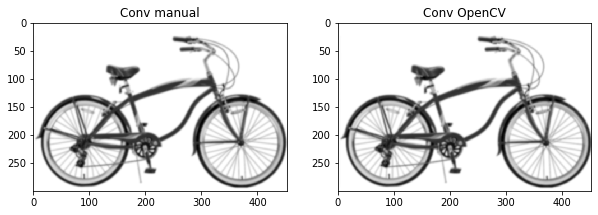
\includegraphics[width=\textwidth]{./imagenes_memoria/bicycle_bifuminada.png}
	\caption{Comparación entre convolución propia (a la derecha) y GaussianBlur (abajo izuierda)}
	\label{conv_propia_vs_openCV}
\end{figure}

\begin{lstlisting}[frame=single]
La intensidad media de la primera imagen es 383.22872489186443 y de la segunda es 383.2287248918644
La diferencia mediana en nivel de gris es de: 0.0 
La diferencia maxima en nivel de gris es de: 5.551115123125783e-16 
La diferencia minima en nivel de gris es de: 0.0 
El numero de pixeles diferentes en la imagen es de: 0
El numero de pixeles diferentes con una diferencia > 1 es de: 0
El numero de pixeles diferentes con una diferencia > 15 es de: 0
La distancia euclídea entre las dos imágenes es de:  3.283706095780364e-14
\end{lstlisting}

Como vemos las dos imágenes son iguales por lo que la implementación de la convolución realizada es correcta. Además para facilitar la corrección de este apartado también he realizado la convolución sobre la matriz de ejemplo que vimos en clase y este es el resultado:

\begin{lstlisting}[frame=single]
Solucion matriz de ejemplo: 

[[210. 360. 330.]
 [520. 800. 680.]
 [570. 840. 690.]]
\end{lstlisting}

Por lo que podemos asegurar que la implementación de la convolución es correcta. También añadir que en el código original hay un bucle por encima del que hace la convolución ya que para el bonus se tenían que tener en cuenta los distintos canales de las imágenes a color. \\

Tras haber convolucionado con una máscara de suavizado la imagen, vamos a hacerlo con las máscaras de derivadas y obtenemos lo siguiente:

\begin{figure}[H]
	\centering
	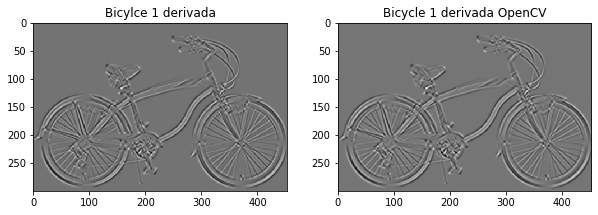
\includegraphics[width=\textwidth]{./imagenes_memoria/conv_1d_bycicle.png}
	\caption{Imagénes convolucionadas con la primera derivada (manualmente a la derecha y con openCV a la izquierda}
	\label{conv_1d_bycicle}
\end{figure}

\begin{figure}[H]
	\centering
	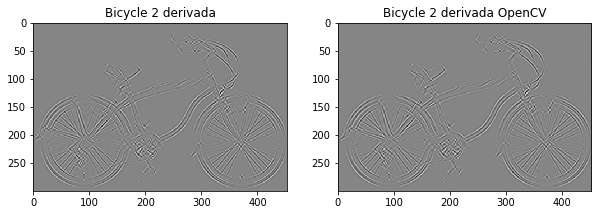
\includegraphics[width=\textwidth]{./imagenes_memoria/conv_2d_bycicle.png}
	\caption{Imagénes convolucionadas con la segunda derivada (manualmente a la derecha y con openCV a la izquierda}
	\label{conv_2d_bycicle}
\end{figure}

Como vemos obtenemos el resultado esperado ya que hemos usado las derivadas de la Gaussiana que son filtros de detección de bordes y es justo lo que observamos en la imagen. Además tanto la solución obtenida por OpenCV como la nuestra son idénticas. 

\subsection{Máscara Laplaciana}
En este ejercicio se nos pide calcular la máscara Laplaciana a partir de una Gaussiana y comparar los resultados con la función Laplaciana de OpenCV. \\

Como sabemos, la máscara Laplaciana es la suma de la convolución por filas con la derivada segunda de la Gaussiana y, luego, por columnas, la convolución con la Gaussiana más la convolución por filas con la Gaussiana y, luego, por columnas, la convolución con la derivada segunda de la Gaussiana, no multiplicamos todo por $\sigma²$ porque ya lo hacemos al calcular las máscaras como vimos anteriormente (\ref{f_laplaciana} para verlo de forma matemática).

\begin{figure}[H]
	\centering
	\[L = (G_{xx}(x,y,\sigma) + G_{yy}(x,y,\sigma)) \]
	\caption{Función Gaussiana.}
	\label{f_laplaciana}
\end{figure}

Por este motivo, de cara a calcular la imagen con la máscara Laplaciana aplicaremos una convolución de la imagen con la máscara de la segunda derivada de la Gaussiana por filas y la máscara Gaussiana por columnas, a esto lo llamaremos $dxx$. Después aplicaremos una convolución a la imagen original con la máscara Gaussiana por filas y la máscara de la segunda derivada de la Gaussiana por columnas, a esto lo llamaremos $dyy$. Finalmente haremos la suma de $dxx$ y $dyy$ y esta será la máscara Laplaciana que devolveremos. \\

Y, calculando la máscara Laplaciana como hemos comentado, obtenemos los siguientes resultados: 

\begin{figure}[H]
	\centering
	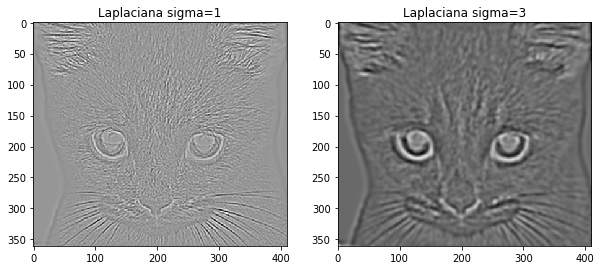
\includegraphics[width=\textwidth]{./imagenes_memoria/comp_sigma_laplaciana.png}
	\caption{Imagen con filtro Laplaciano con $\sigma=1$ a la derecha y $\sigma=3$ a la izquierda)}
	\label{comp_sigma_laplaciana}
\end{figure}

Para hacer la implementación del filtro Laplaciano, OpenCV no utiliza el filtro Gaussiano, utiliza un filtro de Sobel y realiza el mismo cálculo, es decir, calcula la imagen resultante haciendo la suma de la segunda derivada del filtro de Sobel por filas y la suma de la segunda derivada del mismo filtro por columnas. OpenCV genera los siguientes resultados:

\begin{figure}[H]
	\centering
	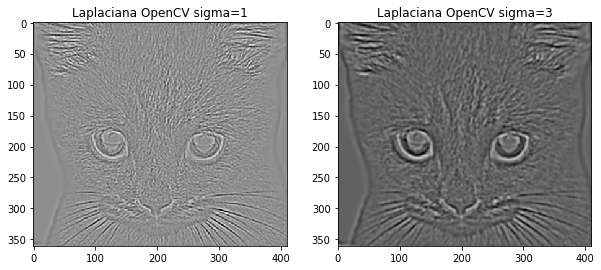
\includegraphics[width=\textwidth]{./imagenes_memoria/com_sigma_laplaciana_opencv.png}
	\caption{Imagen con filtro Laplaciano calculado por OpenCV con $\sigma=1$ a la derecha y $\sigma=3$ a la izquierda)}
	\label{comp_sigma_laplaciana_opencv}
\end{figure}

Como vemos se pueden apreciar diferencias entre las dos imágenes (sobre todo en la imagen con $\sigma=3$) y esto se debe precisamente a que como hemos comentado anteriormente, nosotros hemos calculado la Laplaciana utilizando la máscara Gaussiana mientras que OpenCV lo hace utilizando el filtro de Sobel, por lo tanto es normal que haya algunas diferencias.

\section{Ejercicio 2: Pirámides}
En este ejercicio construiremos dos tipos de pirámides, la Gaussiana y la Laplaciana, y las compararemos con la implementación que realiza OpenCV.

\subsection{Ejercicio 2.1: Pirámide Gaussiana}
En este ejercicio se nos pide crear una pirámide Gaussiana de 4 niveles como mínimo. Una pirámide Gaussiana se construye insertando la imagen original como nivel 0, a esta imagen reducirle el tamaño de alguna manera (en mi caso me quedo con las filas y columnas pares), a la imagen reducida aplicarle convolución y la imagen resultado será la imagén del nivel 1.Para  ello he implementado una función llamada \texttt{piramideGaussiana} que recibe como argumentos la imagen de la que sacar la pirámide , el $\sigma$ que queremos utilizar, los niveles de la pirámide y el tipo de borde a aplicar y devuelve la pirámide Gaussiana.\\

Para crear la pirámide Gaussiana he seguido este esquema:

\begin{itemize}
	\item Inserto la imagen original en la pirámide Gaussiana como el primer nivel (nivel 0).
	\item Genero la máscara Gaussiana con la función \texttt{kernelGaussiano1D} (ejercicio 1A) con el $\sigma$ pasado como argumento.
	\item Para cada nivel realizo los siguientes pasos:
		\begin{itemize}
			\item Añado el padding pasado por argumento a la imagen.
			\item Convoluciono la imagen con la mascara calculada en los pasos anteriores.
			\item Añado la imagen resultante de la convolución a la pirámide como un nuevo nivel.
			\item Me quedo con las filas y las columnas pares para reducir el tamaño de la imagen a la mitad y repetir estos pasos con la nueva imagen.
		\end{itemize}
		
	\item Devuelvo la pirámide
\end{itemize}

Para mostrar todos los niveles de la pirámide he usado la función que concatenaba imágenes de la práctica 0 y he obtenido el resultado de \ref{pir_gauss}\\


Para hacer la comparación con la implementación de pirámide Gaussiana de OpenCV he creado una función llamada \texttt{piramideLaplacianaCV} que recibe como argumentos la imagen sobre la que calcular la pirámide, el número de niveles de la pirámide y el tipo de borde a añadir en la convolución y para crear la pirámide hago los siguientes pasos:

\begin{itemize}
	\item Inserto la imagen original como primer nivel de la pirámide
	\item Para cada nivel utilizo la función \texttt{pyrDown} con el último nivel insertado hasta el momento.
\end{itemize}

Una vez dicho como calculo la pirámide Gaussiana me gustaría aclarar algunas cosas de la función pyrDown de OpenCV:

\begin{itemize}
	\item La función de pyrDown consiste en emborronar una imagen y realizarle un subsample (reducir el tamaño a la imagen).
	\item El emborronado lo hace \textbf{siempre} con la siguiente máscara:
		\begin{figure}[H]
			\centering
			$\begin{pmatrix}
				1 & 4 & 6 & 4 & 1\\
				4 & 16 & 24 & 16 & 4  \\
				6 & 24 & 36 & 24 & 6 \\
				4 & 16 & 24 & 16 & 4 \\
				1 & 4 & 6 & 4 & 1
			\end{pmatrix}$
		\end{figure}
	\item El subsampling lo hace eliminando las columnas y las filas pares.
\end{itemize}

Por tanto, OpenCV calcula las pirámides de manera diferente, sin embargo, yo he usado un $\sigma$ de 1 porque es un estándar y por tanto las pirámides se van a ver casi iguales.

\begin{figure}[H]
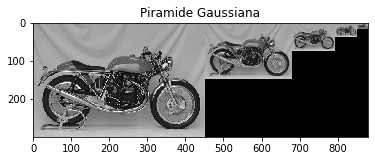
\includegraphics[width=\textwidth]{./imagenes_memoria/pir_gauss.png}
	\caption{Pirámide Gaussiana de la imagen motocycle.bmp}
	\label{pir_gauss}
\end{figure}

\begin{figure}[H]
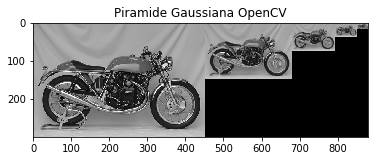
\includegraphics[width=\textwidth]{./imagenes_memoria/pir_gaussCV.png}
	\caption{Pirámide Gaussiana calculada por OpenCV}
	\label{pir_gaussCV}
\end{figure}


Como vemos, en cada nivel, la pirámide se va reduciendo a la mitad en cada nivel (porque en cada nivel nos quedamos solo con las filas y columnas pares) y en cada nivel la imagen se ve más borrosa que en el anterior. Además, como hemos comentado antes, el primer nivel de la pirámide es la imagen original (sin aplicarle ningun filtro). \\

\subsection{Ejercicio 2.2: Pirámide Laplaciana}
En este ejercicio se nos pide crear una pirámide Laplaciana de 4 niveles. Para ello he implementado la función \texttt{piramideLaplaciana} que recibe como parámetros la imagen sobre la que calcular la pirámide, el $\sigma$ que queremos usar, los niveles de las pirámides y por último el tipo de borde para aplicar.

Para crear la pirámide Laplaciana he seguido el siguiente esquema:
\begin{itemize}
	\item Calculo la pirámide Gaussiana.
	\item Para cada nivel aplico los siguientes pasos:
		\begin{itemize}
			\item Almaceno la imagen del siguiente nivel
			\item Le aplico interpolación lineal para aumentarla de tamaño al tamaño de la imagen del nivel en el que nos encontremos.
			\item Resto la imagen de la piramide gaussiana en el nivel actual a la imagen del siguiente nivel con el tamaño cambiado y la imagen resultante será la imagen de la pirámide Laplaciana en ese nivel.
			\item Por último añado el último nivel de la pirámide Gaussiana como el último nivel de la pirámide Laplaciana.
		\end{itemize}
\end{itemize}

Para crear la pirámide Laplaciana con la ayuda de OpenCV he creado la función \\
\texttt{PiramideLaplacianaCV} que recibe como parámetros la imagen a la que calcular la pirámide, el 
número de niveles de la pirámide, y el tipo de borde que añadir para convolucionar la imagen. Para obtener la pirámide Laplaciana hago los siguientes paso:

\begin{itemize}
	\item Calculo la pirámide Gaussiana con la función \texttt{´primadeGaussianaCV}.
	\item Añado como primer nivel la imagen del último nivel de la Gaussiana (voy a crear la pirámide al revés y luego voy a darle la vuelta)
	\item Reescalo la imagen del nivel siguiente (como empezamos desde el final, por ejemplo el siguiente nivel del nivel 3 es el 2) con la función pyrUp de OpenCv.
	\item Restamos la imagen del paso anterior a la imagen de la pirámide Gaussiana del nivel correspondient.
	\item A la pirámide resultante le damos la vuelta y la devolvemos.
\end{itemize}

Antes de presentar los resultados, voy a comentar algunas particularidades del método pyrUp de openCV:

\begin{itemize}
	\item La función de este método es realizar un upsample (aumentar el tamaño) de la imagen pasada como argumento y aplicarle un emborramiento.
	\item El emborronamiento lo calcula con la misma máscara que la de pyrDown pero multiplicada por 4.
	\item El upsample lo realiza inyectando en las posiciones pares filas y columnas de ceros.
\end{itemize}


He obtenido los siguientes resultados:

\begin{figure}[H]
	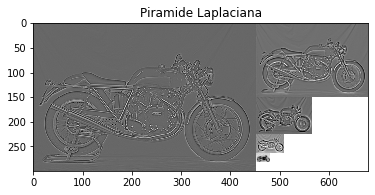
\includegraphics[width=\textwidth]{./imagenes_memoria/pir_lapla.png}
	\caption {Pirámide Laplaciana de la imagen bicycle.bmp}
	\label{pir_lapla}
\end{figure}

\begin{figure}[H]
	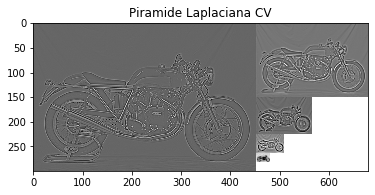
\includegraphics[width=\textwidth]{./imagenes_memoria/pir_laplaCV.png}
	\caption {Pirámide Laplaciana calculada por OpenCV}
	\label{pir_laplaCV}
\end{figure}

Como vemos ambas pirámides son parecidas aunque se calculen de manera diferente porque como hemos explicado anteriormente los $\sigma$ escogidos son parecidos.\\

Además quiero comentar que tuve que implementar una nueva manera de visualizar la pirámide ya que con el método que usé para la pirámide Gaussiana se visualizaba bastante mal la pirámide. Esta función simplemente apila de forma vertical los niveles (a partir del uno) de la pirámide, y apila el nivel cero (imagen horizontal) por la derecha, de forma que el resultado sea una única imagen a mostrar y se visualice de manera correcta.

\subsection{Ejercicio 2.3: Reconstrucción de una imagen}
Con el objetivo de verificar el correcto funcionaminto de la pirámide Laplaciana, se nos pide reconstruir la imagen original a parir de la pirámide Laplaciana. Para hacer esto he creado la función \texttt{reconstruirImagen} que recibe como argumentos la pirámide Laplaciana y los niveles de esta pirámide. Para hacer la reconstrucción de la imagen he seguido el siguiente procedimiento:
\begin{itemize}
	\item Empezando en el último nivel de la pirámide Laplaciana, cogemos la imagen del nivel correspondiente y le aumento el tamaño usando interpolación lineal
	\item A la imagen aumentada le sumo la imagen del siguiente nivel.
	\item Cuando llegamos al último nivel la imagen resultante debe ser la imagen original
\end{itemize}

Siguiendo este procedmiento he obtenido los siguientes resultados:

\begin{figure}[H]
	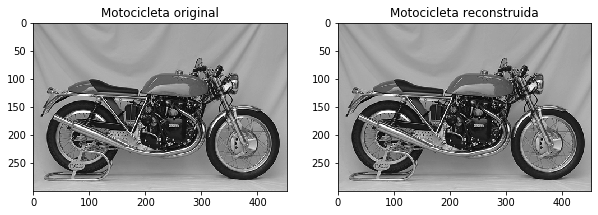
\includegraphics[width=\textwidth]{./imagenes_memoria/reconstruccion_imagen.png}
	\caption{Imagen original a la izquierda e imagen reconstruida a la derecha}
	\label{reconstruccion_imagen}
\end{figure}

Para facilitar la corrección de este ejercicio he implementado una función que calcula los estadísticos de dos imagenes para compararlas mejor. Los resultados obtenidos son:

\begin{lstlisting}[frame=single]
La intensidad media de la primera imagen es 59363.74 y de la segunda es 59363.74
La diferencia mediana en nivel de gris es de: 0.0 
La diferencia maxima en nivel de gris es de: 1.7763568394002505e-14 
La diferencia minima en nivel de gris es de: 0.0 
El numero de pixeles diferentes en la imagen es de: 0
El numero de pixeles diferentes con una diferencia > 1 es de: 0
El numero de pixeles diferentes con una diferencia > 15 es de: 0
La distancia euclidea entre las dos imagenes es de:  1.490341157165124e-13
\end{lstlisting}

Como vemos las imágenes son exactamente iguales, podemos apreciar que hay unas ínfimas diferencias del orden de 10⁻¹⁴ en la distancia euclídea y en la diferencia máxima en nivel de gris. Sin embargo al ser tan pequeñas es casi despreciable y podemos afirmar que las imágenes son iguales.

\section{Bonus: Imágenes Híbridas}
En este ejercicio nos vamos a centrar en crear imágenes híbridas. Una imagen híbrida es una imagen resultado de la  combinación de dos imágenes que admite distintas interpretaciones a distintas distancias.

\subsection{Bonus 1-A: Imágenes híbridas, de altas y bajas frecuencias}
En este ejercicio se nos pide sacar las imágenes de altas y de bajas frecuencias así como las imagen híbrida de dos imagenes. Para conseguir la imagen de bajas frecuencias vamos a utilizar una convolución con una máscara de alisamiento (Gaussiana) y para la imagen de altas frecuencais vamos a usar un filtro Laplaciano. Los $\sigma$ de ambos filtros los eligiremos de manera empírica (probando con varios y viendo los resultados), para la imagen híbrida simplemente sumaremos la imagen de bajas frecuencias más la imagen de altas frecuencias (ambas normalizadas). Para mostrar las 3 imágenes usaremos la función para visualizar imágenes de la práctica 0. El resultado que he obtenido es el siguiente:

\begin{figure}[H]
	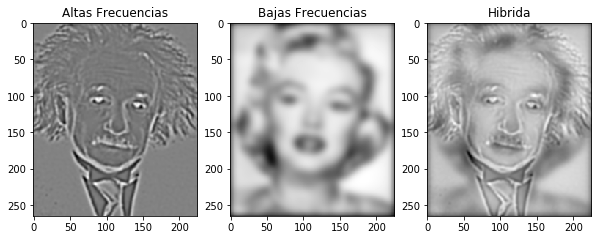
\includegraphics[width=\textwidth]{./imagenes_memoria/b1a.png}
	\caption{Imagen de altas frecuencias de Albert Einstein a la izquierda, en el medio imagen de bajas frecuencias de Marilyn Monroe y a la derecha la imagen híbrida}
	\label{bonus1a} 
\end{figure}

Para obtener esta figura he utilizado un $\sigma$ de 2 para la imagen de altas frecuencias y un $\sigma$ de 5 para la imagen de bajas frecuencias. Para la imagen de altas frecuncias he probado con valores de $\sigma$ de 7,5,3 y 2 y para la imagen de bajas frecuencias he probado con valores d $\sigma$ de 6,8,4 y 5. He decidido quedarme con los valores 2 y 5 porque de esta manera Einstein no se predomina de una manera apabullante frente a Marilyn y se logra un efecto conseguido.

\subsection{Bonus 1-B: Creando más imágenes híbridas}
En este ejercicio se nos pide repetir el apartado anterior pero con 3 parejas de imágenes distintas. \\

La primera pareja de imágenes que he escogido ha sido la imagen del pájaro y la del avión. He seleccionado al pájaro como imagen de altas frecuencias y al avión como bajas frecuencias y les he aplicado sus filtros con un valor de $\sigma$ de 3 y 6 respectivamente. Para este par de imágenes empecé usando valores de $\sigma$ de 2 y 5 porque fueron los que elegimos para el apartado anterior y rápidamente nos dimos cuenta de que el pájaro debía de verse más y el avión un poco menos por lo que aumentamos el valor de $\sigma$ en uno en ambos filtros y dimos con el siguiente resultado:

\begin{figure}[H]
	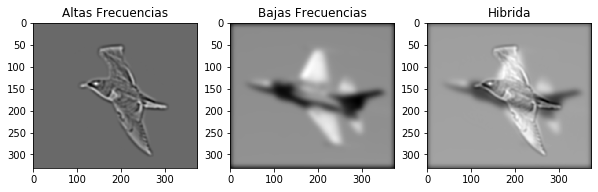
\includegraphics[width=\textwidth]{./imagenes_memoria/b1b}
	\caption{Imagen de altas frecuencias del pájaro a la izquierda, en el medio imagen de bajas frecuencias del avión y a la derecha la imagen híbrida}
	\label{bonus1ba}
\end{figure}
	
La segunda pareja de imágenes que he escogido ha sido la imagen del pez y la del submarino. He seleccionado al pez como imagen de altas frecuencias y al submarino como bajas frecuencias y les he aplicado sus filtros con un valor de $\sigma$ de 2 y 8 respectivamente. Para este par de imágenes empecé usando valores de $\sigma$ de 3 y 6 porque fueron los que elegimos para el apartado anterior y al ver que el pez se visualizaba bien pero el submarino se visualizaba de más fui aumentando el $\sigma$ del submarino hasta dar con el siguiente resultado:

\begin{figure}[H]
	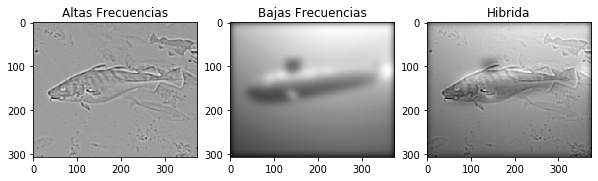
\includegraphics[width=\textwidth]{./imagenes_memoria/bonus1bb}
	\caption{Imagen de altas frecuencias del pájaro a la izquierda, en el medio imagen de bajas frecuencias del submarino y a la derecha la imagen híbrida}
	\label{bonus1bb}
\end{figure}
	

Para la última pareja de imágenes que he escogido ha sido la imagen del gato y la del perro. He seleccionado al gato como imagen de altas frecuencias y al perro como bajas frecuencias y les he aplicado sus filtros con un valor de $\sigma$ de 2 y 5 respectivamente. Para este par de imágenes he probado con muchos valores de $\sigma$ (del 1 al 10) y me he quedado con el 2 y el 5 que aunque el resultado no sea tan satisfactorio como en las anteriores parejas de imágenes lo considero un resultado aceptable.

\begin{figure}[H]
	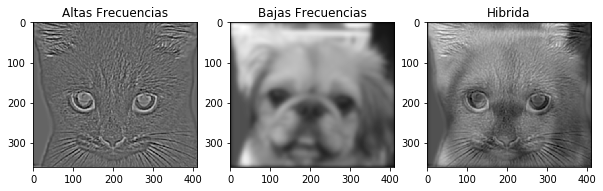
\includegraphics[width=\textwidth]{./imagenes_memoria/b1bc}
	\caption{Imagen de altas frecuencias del gato a la izquierda, en el medio imagen de bajas frecuencias del perro y a la derecha la imagen híbrida}
	\label{bonus1bc}
\end{figure}

\subsection{Bonus 1-C: Pirámides Gaussianas de las imágenes híbridas}
En este ejercicio se nos pide crear las pirámides Gaussianas de las imagenes híbridas del apartado anterior. Para hacer esto me he servido de las funciones creadas en apartados anteriores tanto para crear la pirámide Gaussiana como para visualizarla. A la hora de calcular la pirámide Gaussiana he utilizado un $\sigma$ de 1 ya que como hemos dicho antes es un estándar y de esta manera las imágenes no se emborronan tanto y se puede apreciar el efecto claramente.

\begin{figure}[H]
	\centering
	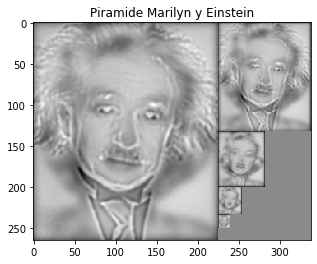
\includegraphics[scale=1.1]{./imagenes_memoria/b1ca}
	\caption{Pirámide Gaussiana Marilyn-Einstein}
	\label{bonus1ca}
\end{figure}

\begin{figure}[H]
	\centering
	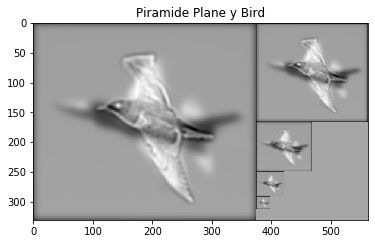
\includegraphics[scale=1.1]{./imagenes_memoria/b1cb}
	\caption{Pirámide Gaussiana Avión-Pájaro}
	\label{bonus1cb}
\end{figure}

\begin{figure}[H]
	\centering
	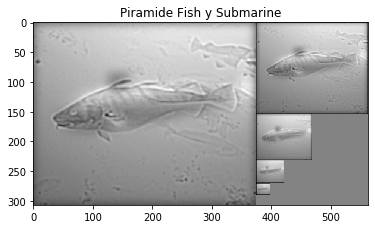
\includegraphics[scale=1.1]{./imagenes_memoria/b1cc}
	\caption{Pirámide Gaussiana Pez-Submarino}
	\label{bonus1cc}
\end{figure}

\begin{figure}[H]
	\centering
	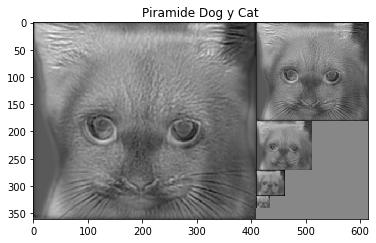
\includegraphics[scale=1.1]{./imagenes_memoria/b1cd}
	\caption{Pirámide Gaussiana Gato-Perro}
	\label{bonus1cd}
\end{figure}

Como vemos se observa el efecto del que hablamos en la introducción de esta sección, en las imágenes más grandes (con menos nivel de emborronamiento) se observa con más facilidad la imagen de altas frecuencias (como si estuviésemos muy cerca de la imagen) y conforme la imagen se va haciendo más pequeña la imagen de bajas frecuencias se hace cada vez más visible hasta que la de altas frecuencias es invisible (efecto de ir alejandote cada vez más de la imagen)


\subsection{Bonus 2: Imágenes híbridas a color}
En este ejercicio se nos pide realizar lo mismo que en el anterior pero con las imágenes a color. Para ello simplemente tenemos que hacer modificaciones en nuestra implementación de la convolución para que esta en haga lo mismo que en el ejercicio 1C pero que lo haga sobre cada canal y leer la imagen con el flag de color activo. Una vez hechos estos cambios utilizamos los mismos parámetros y  el mismo método que en el apartado anterior  y obtenemos los siguientes resultados:

\begin{figure}[H]
	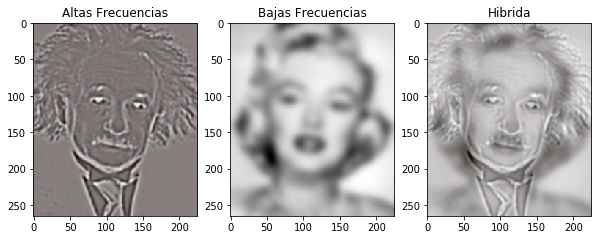
\includegraphics[width=\textwidth]{./imagenes_memoria/b2a1}
	\caption{Imagen de altas frecuencias de Einstein a la izquierda, en el medio imagen de bajas frecuencias de Marilyn y a la derecha la imagen híbrida}
	\label{bonus2a1}
\end{figure}

\begin{figure}[H]
	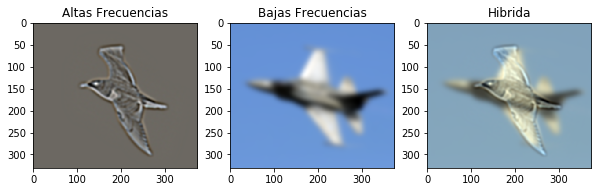
\includegraphics[width=\textwidth]{./imagenes_memoria/b2b1}
	\caption{Imagen de altas frecuencias del pájaro a la izquierda, en el medio imagen de bajas frecuencias del avión y a la derecha la imagen híbrida}
	\label{bonus2b1}
\end{figure}

\begin{figure}[H]
	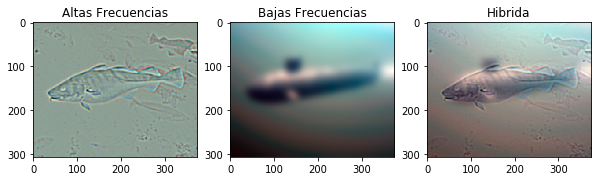
\includegraphics[width=\textwidth]{./imagenes_memoria/b2c1}
	\caption{Imagen de altas frecuencias del pez a la izquierda, en el medio imagen de bajas frecuencias del submarino y a la derecha la imagen híbrida}
	\label{bonus2c1}
\end{figure}

\begin{figure}[H]
	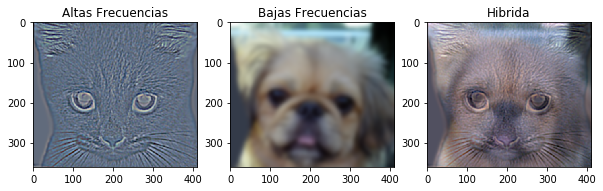
\includegraphics[width=\textwidth]{./imagenes_memoria/b2d1}
	\caption{Imagen de altas frecuencias del gato a la izquierda, en el medio imagen de bajas frecuencias del perro y a la derecha la imagen híbrida}
	\label{bonus2d1}
\end{figure}

\begin{figure}[H]
	\centering
	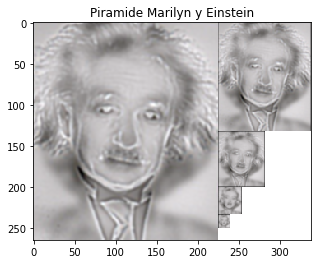
\includegraphics[scale=1.1]{./imagenes_memoria/b2a2}
	\caption{Pirámide Gaussiana Marilyn-Einstein a color}
	\label{bonus2a}
\end{figure}

\begin{figure}[H]
	\centering
	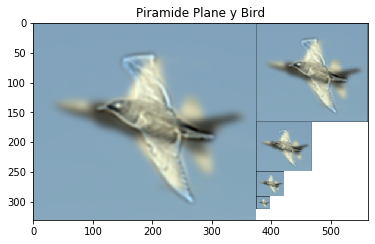
\includegraphics[scale=1.1]{./imagenes_memoria/b2b2}
	\caption{Pirámide Gaussiana Avión-Pájaro a color}
	\label{bonus2b}
\end{figure}

\begin{figure}[H]
	\centering
	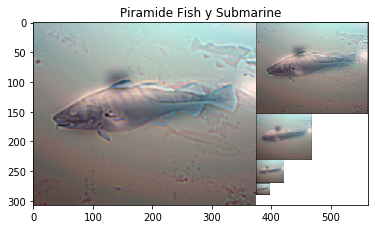
\includegraphics[scale=1.1]{./imagenes_memoria/b2c2}
	\caption{Pirámide Gaussiana Pez-Submarino a color}
	\label{bonus2c}
\end{figure}

\begin{figure}[H]
	\centering
	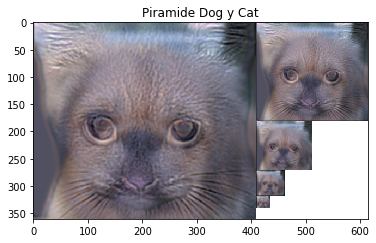
\includegraphics[scale=1.1]{./imagenes_memoria/b2d2}
	\caption{Pirámide Gaussiana Gato-Perro a color}
	\label{bonus2d}
\end{figure}

\subsection{Bonus 3: Imagen Híbrida con imagen a nuestra elección}
En este ejercicio se nos pide crear una imagen híbrida eligiendo dos imágenes a nuestra elección. Para elegir la pareja de imágenes he mirado la literatura y me he encontrado muchos ejemplos mezclando con el par de imágenes de Mr Bean y de José Luis Rodríguez Zapatero y por ello he decidido usarlas porque se consigue un efecto logrado. Para realizar la imagen híbrida sigo los mismos pasos que en los apartados anteriores eligiendo un $\sigma$ (de manera empírica probando valores, en este caso empecé con $\sigma=1$ para las altas frecuncias y 2 para las bajas y fui subiendo hasta que di con un resultado satisfactorio) de 1.5 para la imágen de altas frecuencias (Zapatero) y con un $\sigma$ de 4 para la imágen de bajas frecuencias (Mr Bean) y he obtenido los siguientes resultados:

\begin{figure}[H]
	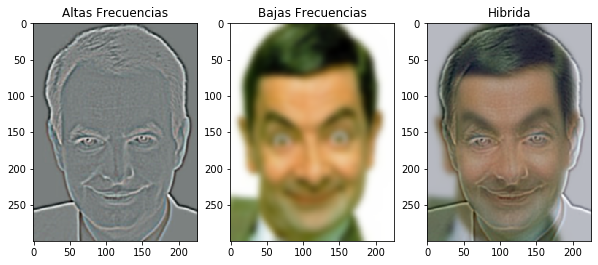
\includegraphics[width=\textwidth]{./imagenes_memoria/b3a}
	\caption{Imagen de altas frecuencias de Einstein a la izquierda, en el medio imagen de bajas frecuencias de Marilyn y a la derecha la imagen híbrida}
	\label{bonus31}
\end{figure}

\begin{figure}[H]
	\centering
	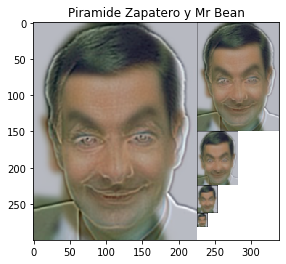
\includegraphics[scale=1.1]{./imagenes_memoria/b3b}
	\caption{Pirámide Gaussiana MrBean-Zapatero a color}
	\label{bonus3b}
\end{figure}

\section{Bibliografía}


\begin{thebibliography}{9}

\bibitem{bordertypes}
	Border types - Documentación oficial de OpenCV.

	\url{https://docs.opencv.org/4.4.0/d2/de8/group__core__array.html#ga209f2f4869e304c82d07739337eae7c5}

\bibitem{separabilidad_2D}
	Prueba de separabilidad para las convoluciones 2D.

	\url{https://www.songho.ca/dsp/convolution/convolution2d_separable.html}

\bibitem{getDerivKernelsCV}
	getDerivKernels - Documentación oficial de OpenCV.

	\url{https://docs.opencv.org/4.4.0/d4/d86/group__imgproc__filter.html#ga6d6c23f7bd3f5836c31cfae994fc4aea}


\bibitem{copyborder}
	copyMakeBorder - Documentación oficial de OpenCV.

	\url{https://docs.opencv.org/4.4.0/d2/de8/group__core__array.html#ga2ac1049c2c3dd25c2b41bffe17658a36}

\bibitem{pyrUpCV}
	pyrUp - Documentación oficial de OpenCV.

	\url{https://docs.opencv.org/4.4.0/d4/d86/group__imgproc__filter.html#gada75b59bdaaca411ed6fee10085eb784}

\bibitem{pyrDownCV}
	pyrDown - Documentación oficial de OpenCV.

	\url{https://docs.opencv.org/4.4.0/d4/d86/group__imgproc__filter.html#gaf9bba239dfca11654cb7f50f889fc2ff}

\bibitem{img_hibridas}

	A. Oliva, A. Torralba, P.G. Schyns(2006). Hybrid Images. ACM Transactions onGraphics.

	\url{http://olivalab.mit.edu/hybridimage.htm}


\end{thebibliography}

\end{document}
